\chapter{Manuale Utente}
\label{chapter3}
In questo capitolo verranno presentate tutte le schermate che concernono l'applicazione e le varie funzioni di ognuna.
\\Più precisamente, nella sezione \ref{mappa} verrà presentata la prima schermata che l'utente incontra quando apre l'applicazione per la prima volta, nella sezione \ref{homepage} verrà presentata la schermata principale dell'applicazione, nella sezione \ref{notavocale} verrà presentata la schermata che riguarda la registrazione della nota vocale, nella sezione \ref{notascritta} verrà presentata la schermata che riguarda l'inserimento della nota scritta.
\\Successivamente, nelle sezioni \ref{modificafoto}, \ref{modificavideo}, \ref{modificavocale}, verranno presentate le schermate addette al compito di modificare i file multimediali registrati fino a quel momento.

\section{Mappa}
\label{mappa}
Quando l'utente apre l'applicazione per la prima volta, gli verrà richiesto di accettare i permessi, come si può vedere in figura \ref{fig:permessiPosizione}:
\begin{figure}[!h]
    \centering
	
\includegraphics[scale=0.115]{Tesi/images/PermessiPosizione}
	\caption{\textit{Permessi posizione}}
	\label{fig:permessiPosizione}
\end{figure}\pagebreak
\\Accettando i permessi, sarà possibile caricare e visualizzare la mappa e geolocalizzare il dispositivo, come si può vedere in figura \ref{fig:mappa}, che si riferisce al layout \textit{activity\_maps.xml}:
\begin{figure}[!h]
    \centering
	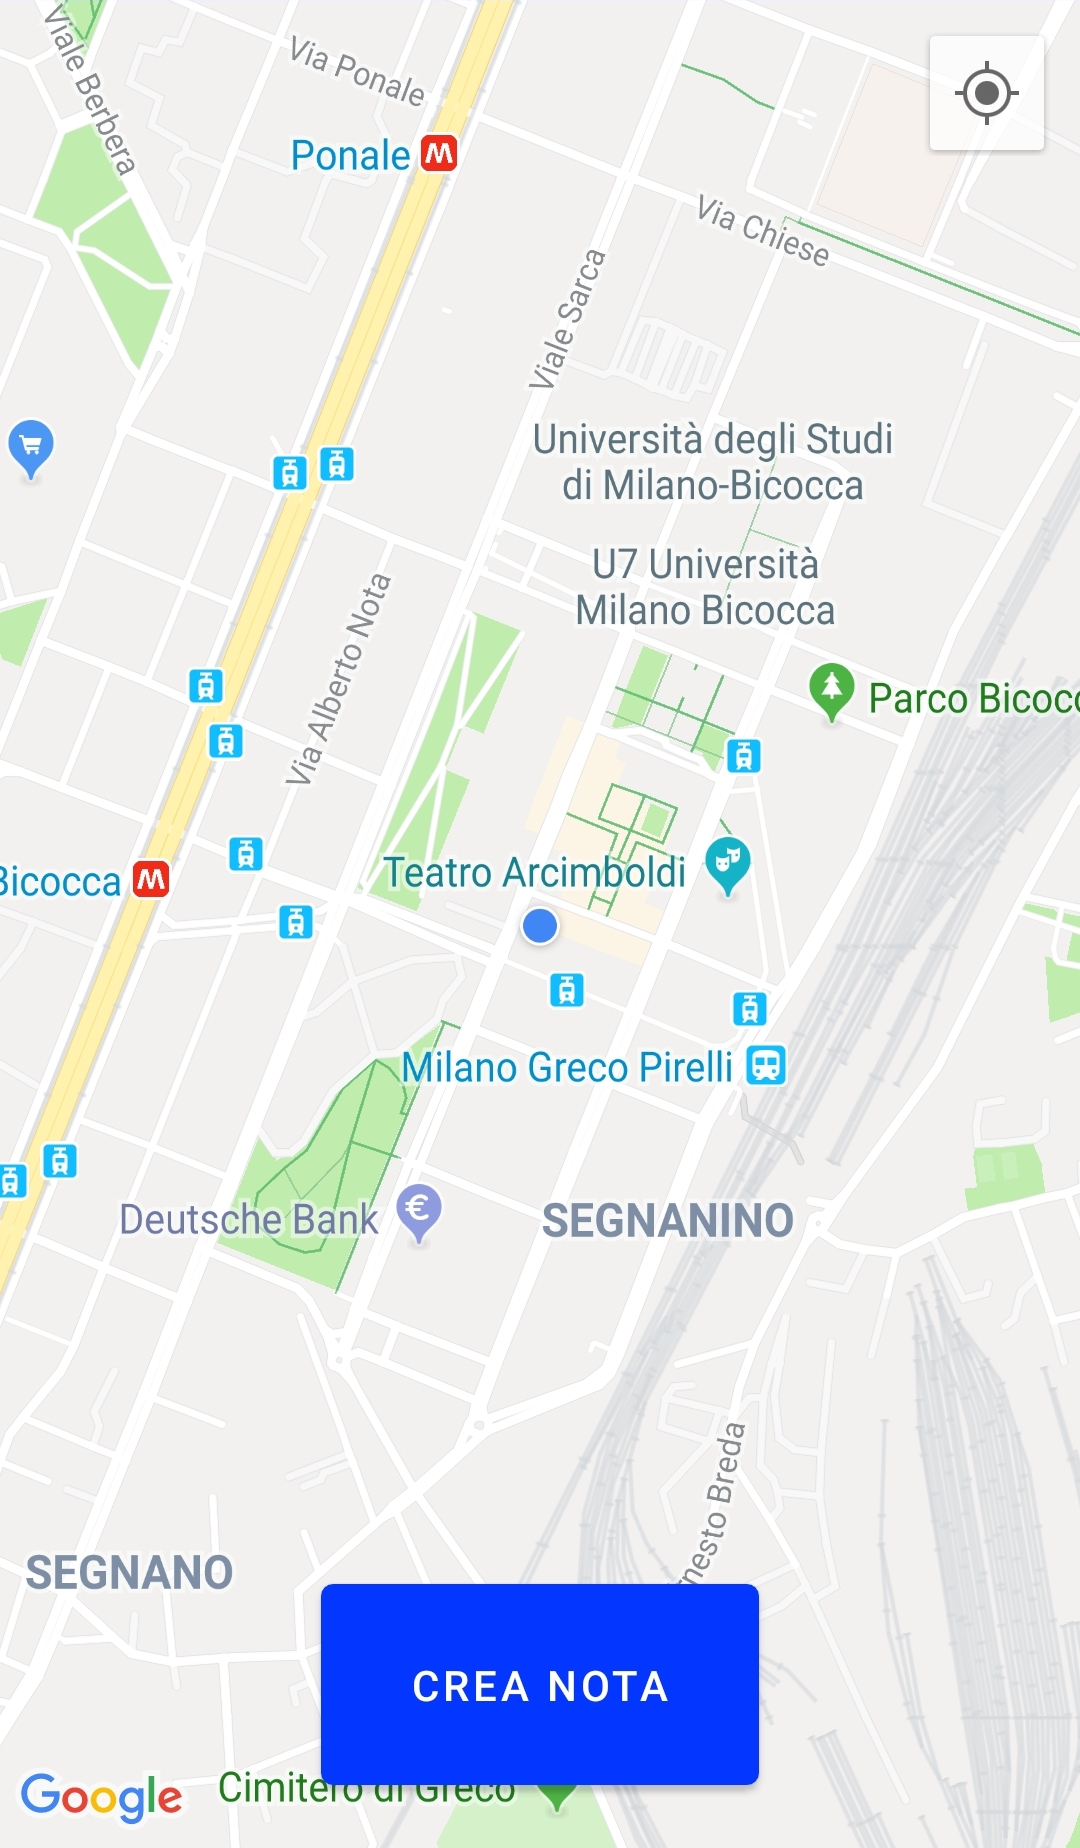
\includegraphics[scale=0.15]{Tesi/images/Mappa.jpg}
	\caption{\textit{Mappa}}
	\label{fig:mappa}
\end{figure}
\\All'interno di questa schermata, l'utente, potrà muoversi all'interno della mappa, schiacciare sul bottone "Crea Nota" oppure geolocalizzarsi sulla posizione corrente, cliccando il bottone in alto a destra.
\\Se, nel caso il dispositivo non riesca a recuperare la posizione, comparirà un messaggio che avviserà l'utente che si sta provando a caricare la posizione. Questo comportamento si può notare nella figura \ref{fig:snackposizione}.
\begin{figure}[!h]
    \centering
	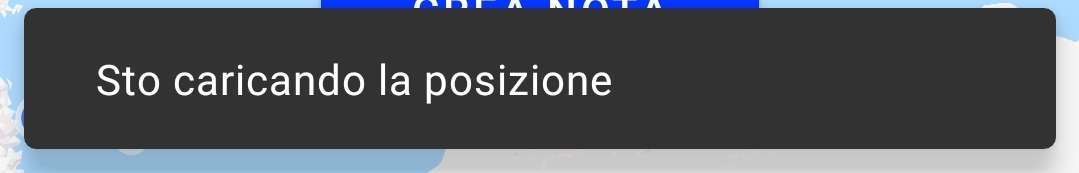
\includegraphics[scale=0.3]{Tesi/images/SnackPosizione}
	\caption{\textit{Snackbar posizione non recuperata}}
	\label{fig:snackposizione}
\end{figure}
\\Se per caso l'utente avesse già aperto l'applicazione in precedenza, e avesse già accettato i permessi, la prima schermata dell'applicazione si presenterebbe direttamente con la mappa come in figura \ref{fig:mappa}.
\pagebreak

\section{Homepage}
\label{homepage}
La schermata principale dell'applicazione è questa che si può vedere in figura \ref{fig:homepage}, che si riferisce al layout \textit{activity\_post.xml}:
\begin{figure}[!h]
    \centering
	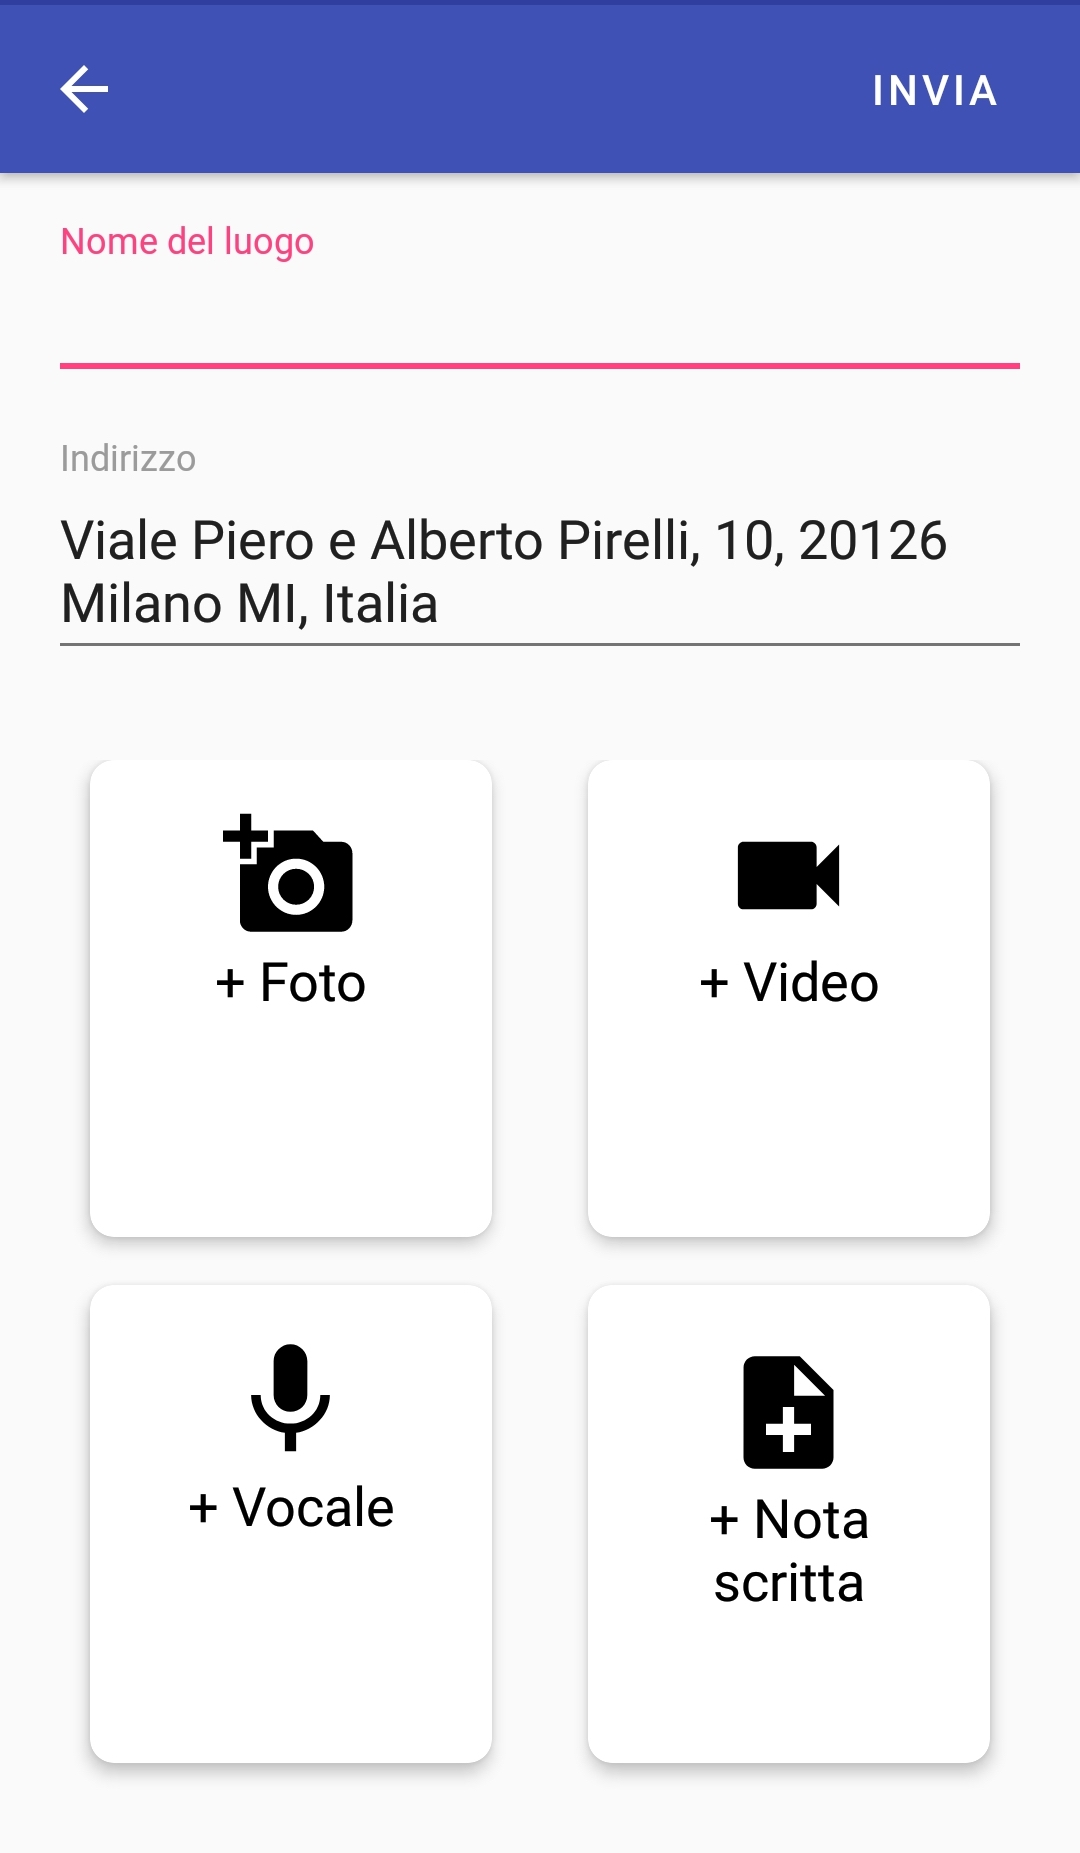
\includegraphics[scale=0.15]{Tesi/images/Homepage.jpg}
	\caption{\textit{Homepage}}
	\label{fig:homepage}
\end{figure}
\\Se è il primo avvio dell'applicazione, verrà chiesto all'utente di accettare i permessi relativi alla scrittura e alla lettura in memoria del dispositivo, come si può vedere in figura \ref{fig:permessimem}:
\begin{figure}[!h]
    \centering
	
\includegraphics[scale=0.25]{Tesi/images/PermessiMemoria.jpg}
	\caption{\textit{Permessi memoria}}
	\label{fig:permessimem}
\end{figure}\pagebreak
\\Come si può osservare dalla figura \ref{fig:homepage}, l'indirizzo verrà popolato in maniera automatica se il dispositivo riuscirà a recuperare la posizione corrente del dispositivo.
\\In questa schermata l'utente avrà la libertà di scattare foto, registrare video, registrare note audio e scrivere una nota scritta. Inoltre potrà inserire il nome del luogo in cui si trova, che sceglierà a sua discrezione.
\\Come si può vedere dalla figura \ref{fig:homepagemodifica}, una volta che è stato inserito almeno un elemento, appartenente ad una determinata categoria, verrà anche visualizzato un bottone "Modifica" ed un numero che corrisponde al numero di elementi presenti fino a quel momento:
\begin{figure}[!h]
    \centering
	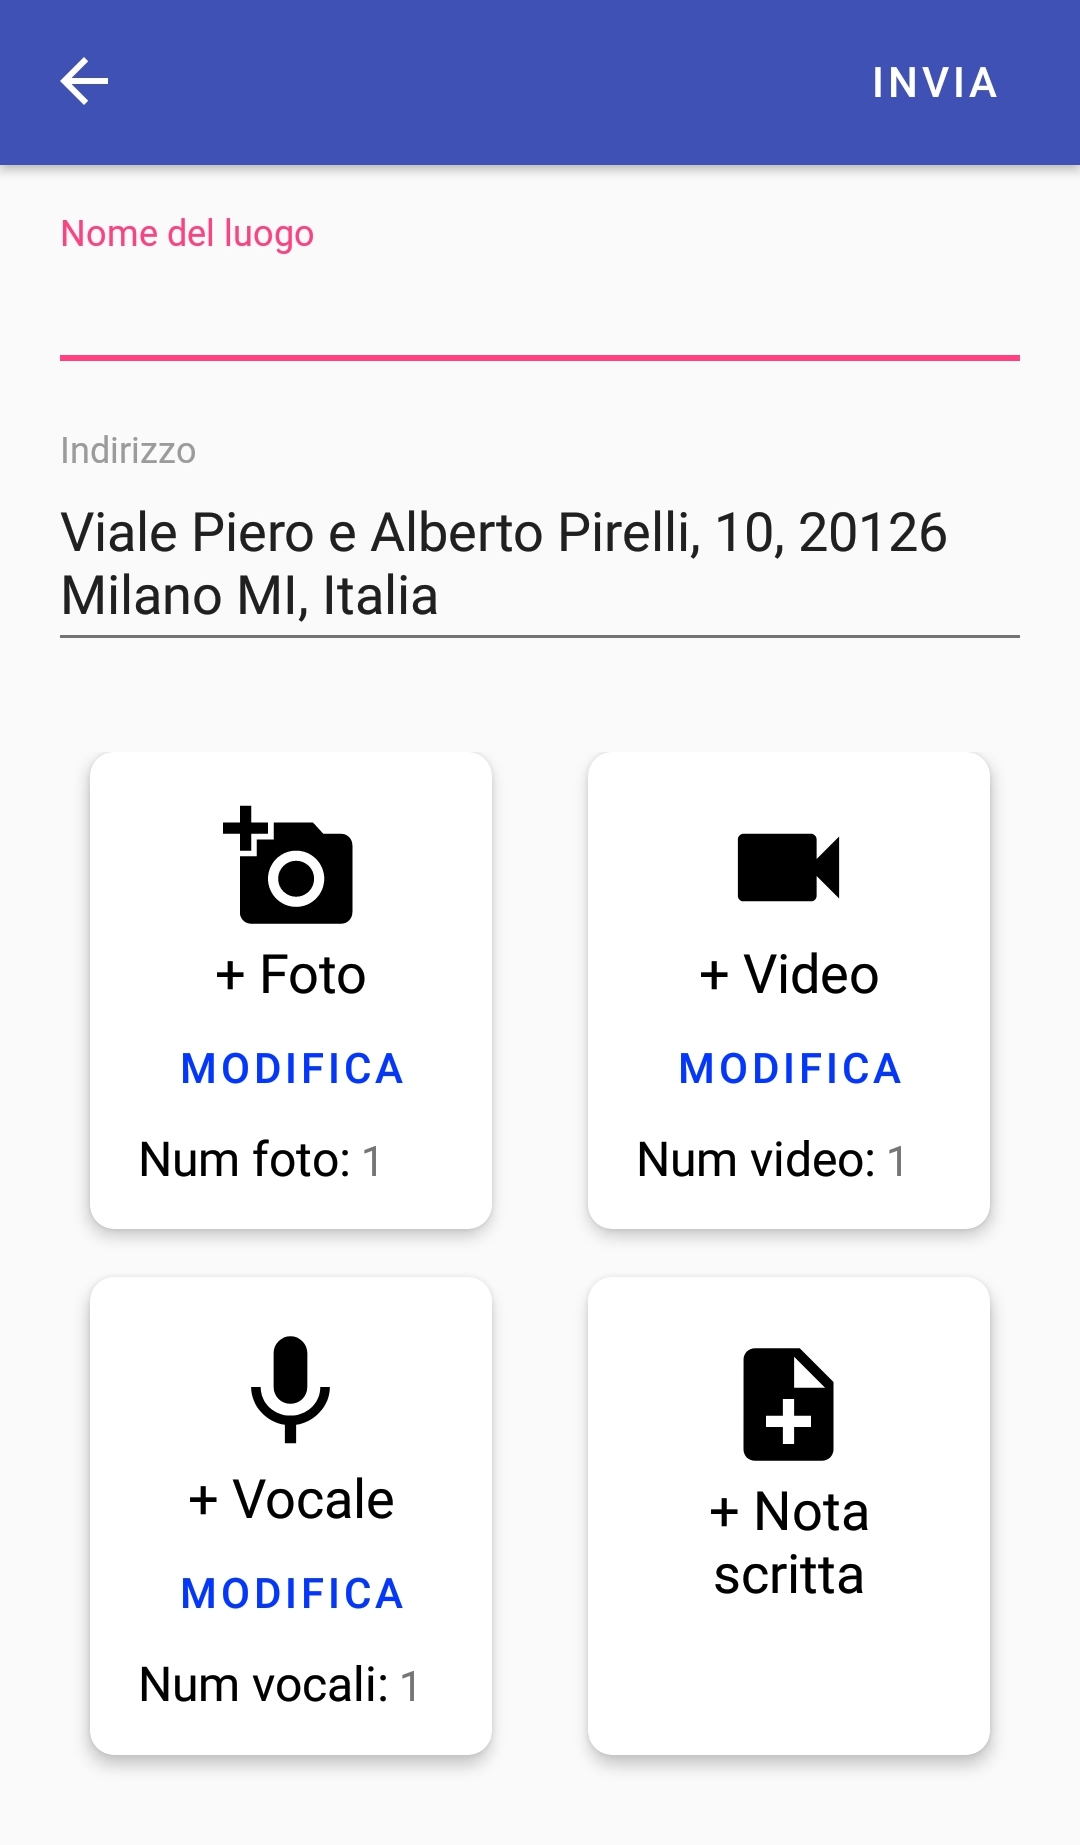
\includegraphics[scale=0.15]{Tesi/images/HomepageModifica.jpg}
	\caption{\textit{Homepage con tasto modifica}}
	\label{fig:homepagemodifica}
\end{figure}
\\E' presente una toolbar in alto alla schermata, dove a sinistra l'utente potrà tornare indietro, nella schermata della mappa, schiacciando sulla freccia direzionata verso sinistra, ed a destra, è presente il tasto "invia", che permetterà all'utente di inviare ciò che ha scattato/registrato, al repository centralizzato.
\\Inoltre, se sono presenti degli elementi all'interno della nota, e l'utente decidesse di tornare indietro, senza aver inviato i dati, verrà avvisato tramite un messaggio che gli chiederà se è sicuro di tornare indietro, poichè, in caso positivo, perderebbe i dati acquisiti fino a quel momento.
\\Questo comportamento si può osservare in figura \ref{fig:alerthomepage}:
\begin{figure}[!h]
    \centering
	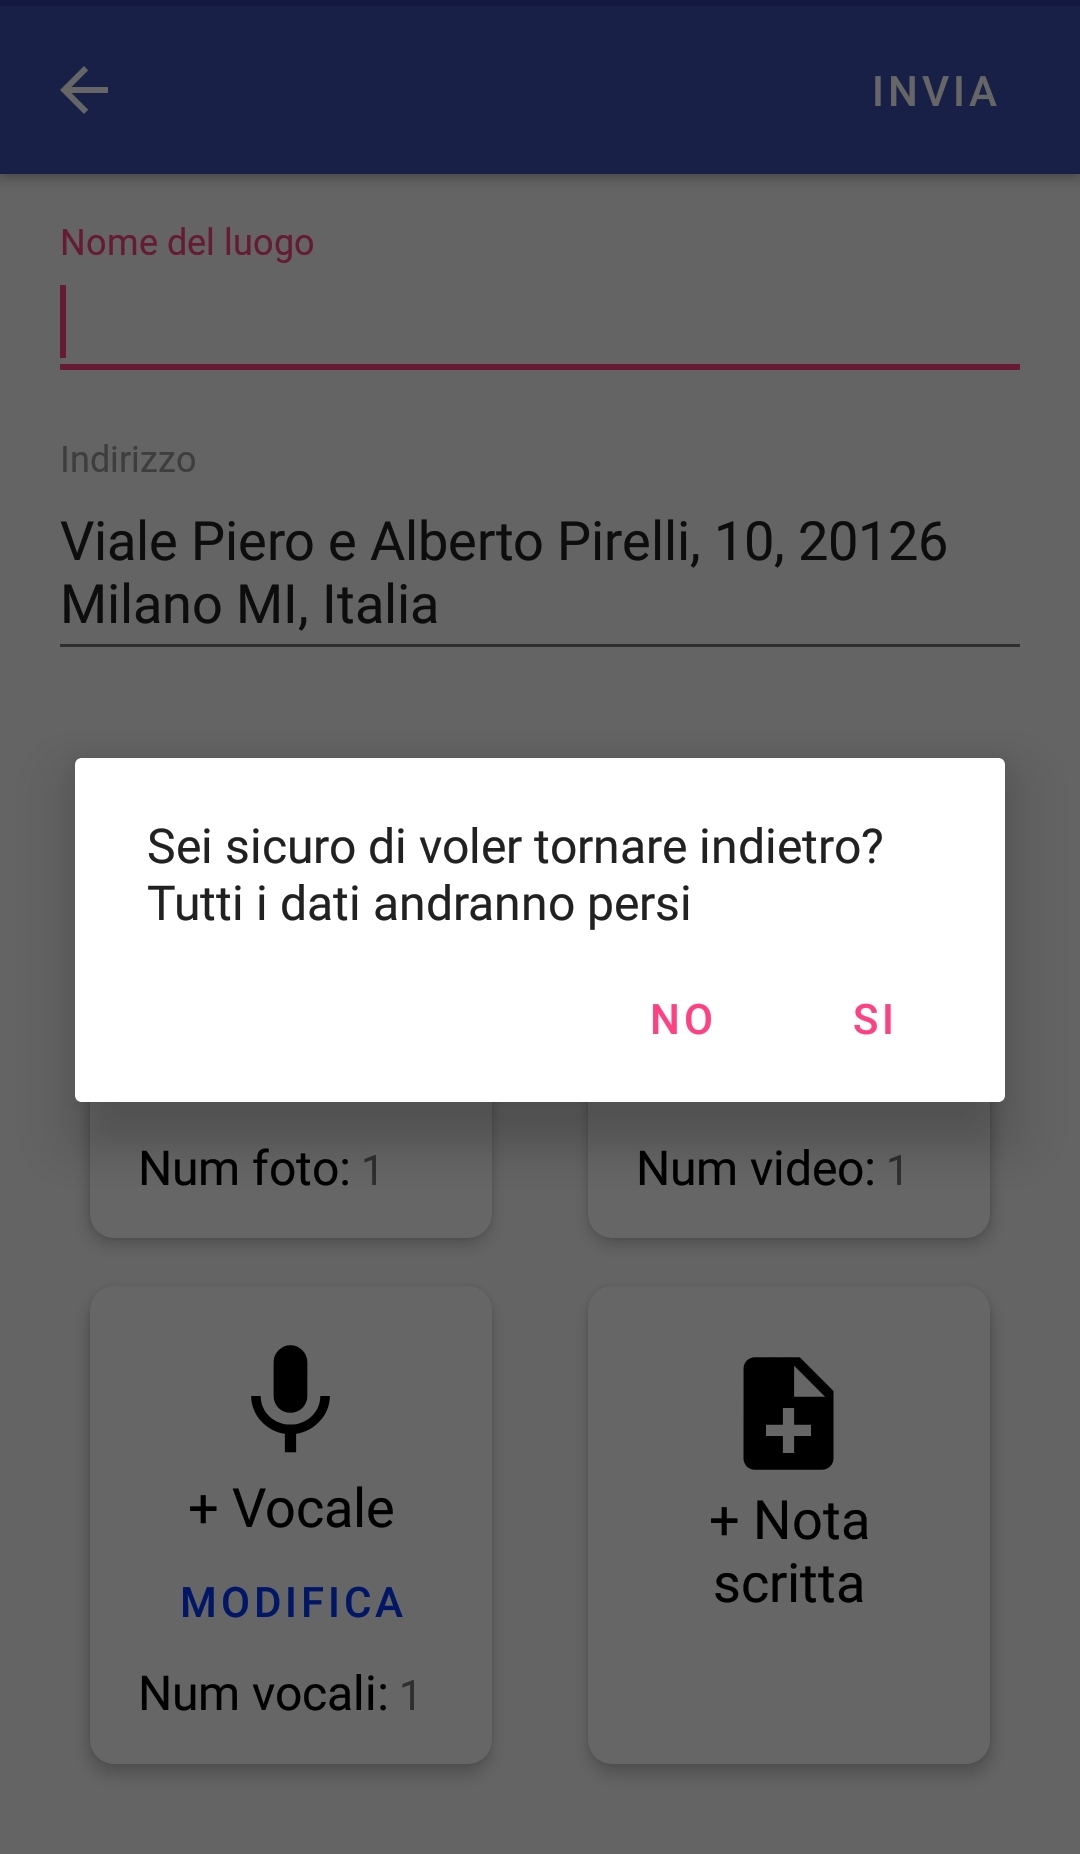
\includegraphics[scale=0.15]{Tesi/images/AlertHomepage}
	\caption{\textit{Alert Homepage}}
	\label{fig:alerthomepage}
\end{figure}\pagebreak
\\Dopodichè, quando l'utente schiaccerà sul tasto "Invia" verrà mostrato un messaggio che darà all'utente un feedback sul progresso del caricamento dei dati sul repository centralizzato.
\\Questo comportamento si può vedere in figura \ref{fig:progresso}:
\begin{figure}[!h]
    \centering
	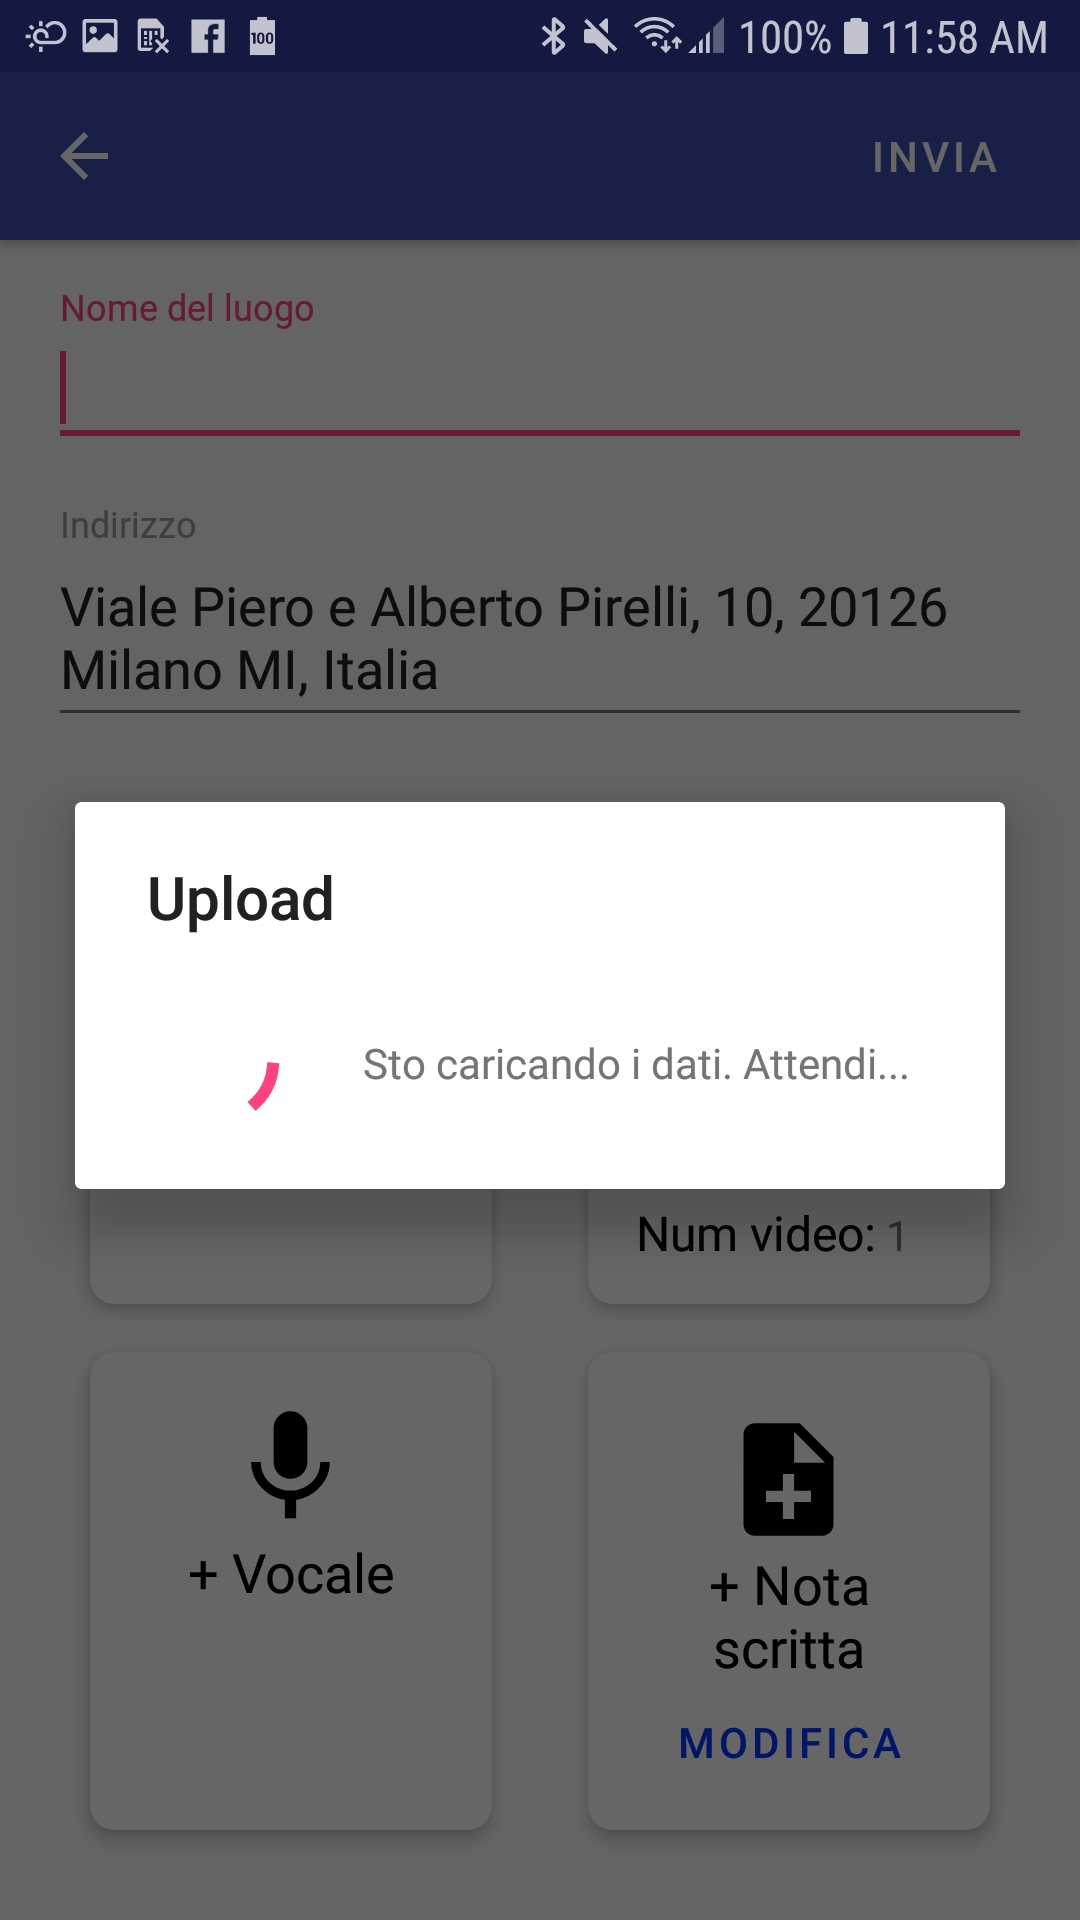
\includegraphics[scale=0.135]{Tesi/images/Progresso}
	\caption{\textit{Progresso durante il caricamento}}
	\label{fig:progresso}
\end{figure}\pagebreak
\\Una volta che sarà finito il caricamento, l'applicazione tornerà alla schermata principale, ovvero quella della mappa in figura \ref{fig:mappa}.
\\Una volta che l'applicazione sarà tornata nella schermata della mappa, verrà visualizzato un messaggio che darà un feedback all'utente che il caricamento sarà avvenuto con successo.
\\Questo comportamento si può osservare nella figura \ref{fig:snackcaricamento}:
\begin{figure}[!h]
    \centering
	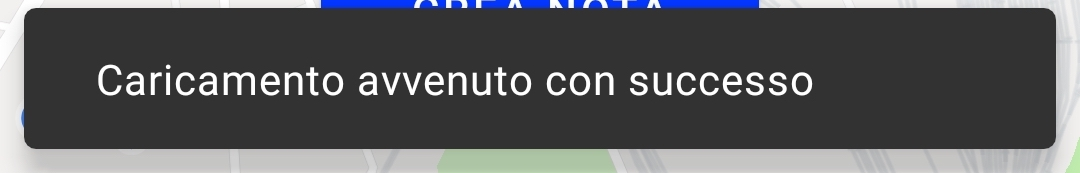
\includegraphics[scale=0.3]{Tesi/images/SnackCaricamento}
	\caption{\textit{Snackbar caricamento}}
	\label{fig:snackcaricamento}
\end{figure}

\section{Nota vocale}
\label{notavocale}
All'interno di questa schermata, si possono osservare due bottoni che permettono di avviare e terminare una registrazione vocale.
\\Si può osservare l'aspetto di questa schermata in figura \ref{fig:notavocale}, che si riferisce al layout \textit{activity\_microphone.xml}:
\begin{figure}[!h]
    \centering
	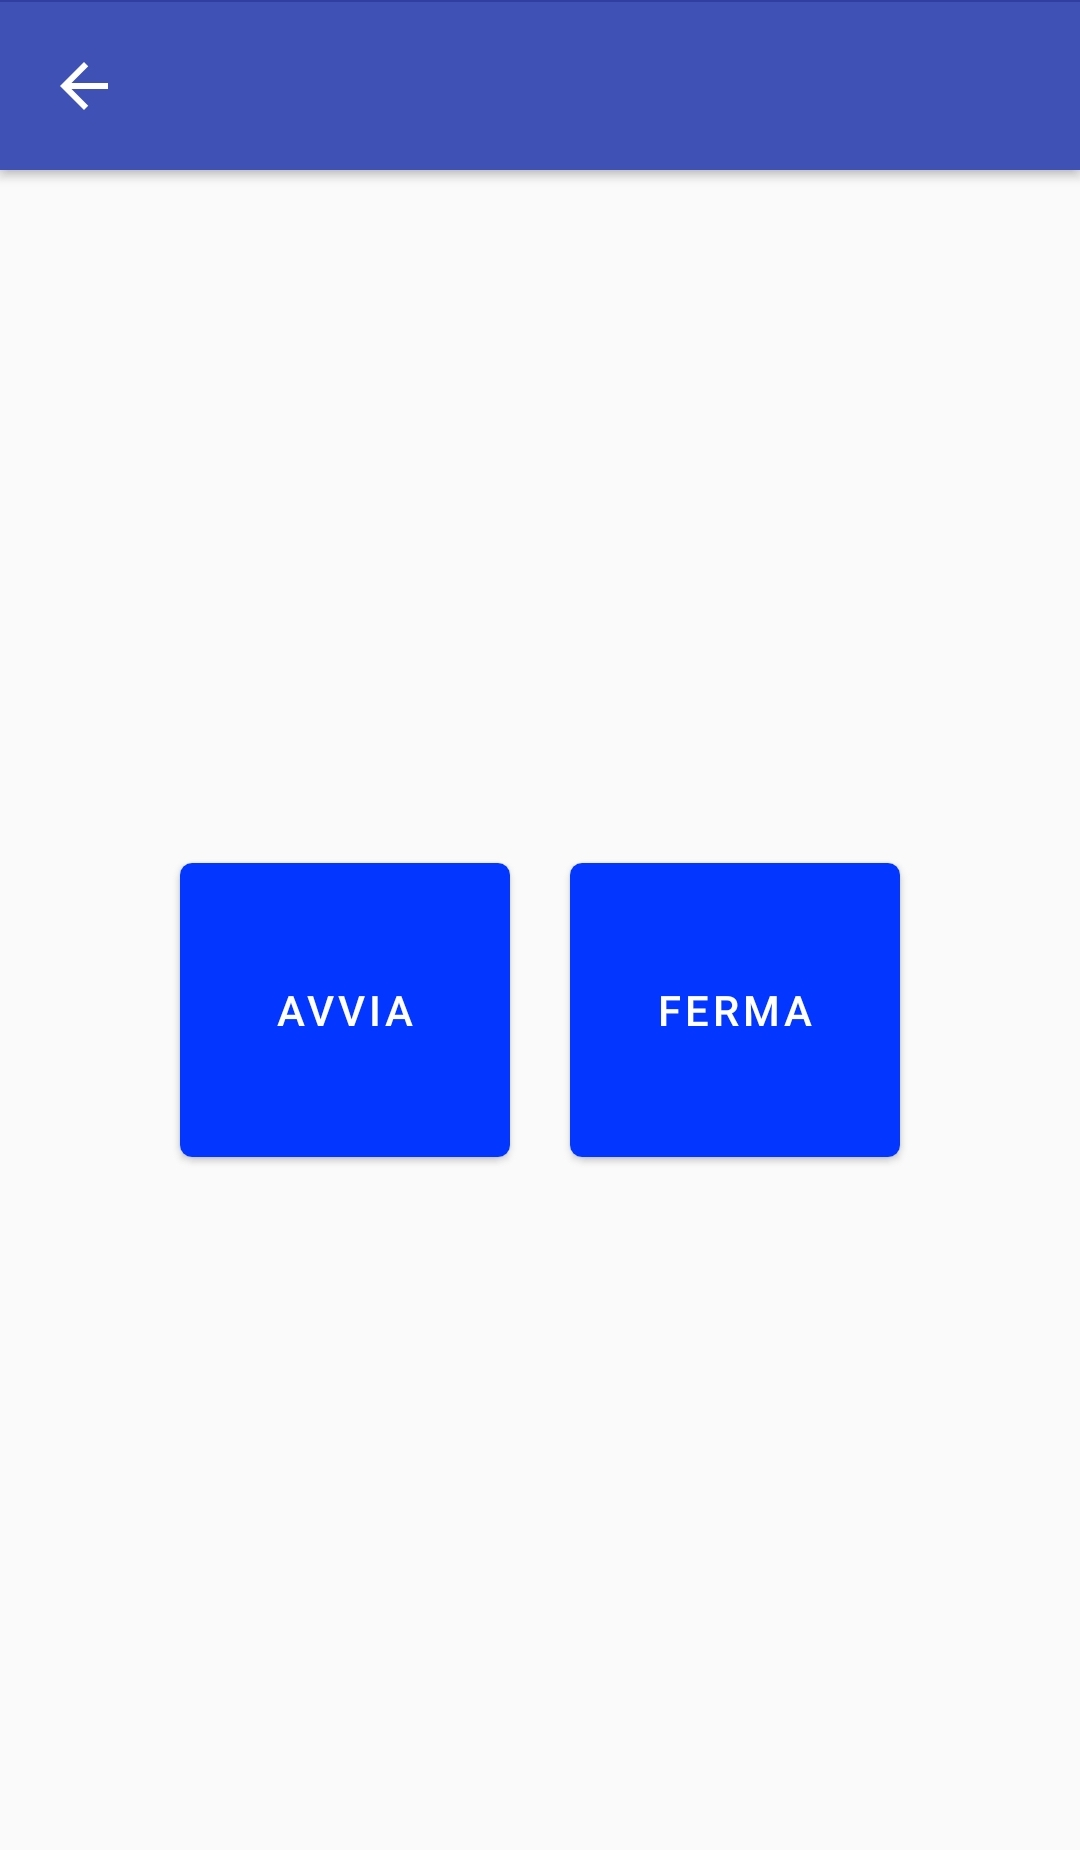
\includegraphics[scale=0.14]{Tesi/images/AttVocale.jpg}
	\caption{\textit{Schermata nota vocale}}
	\label{fig:notavocale}
\end{figure}
\\Con il tasto a sinistra si avvia la registrazione, e verrà mostrata una barra di progressione sopra questi due bottoni, che darà un feedback all'utente che la registrazione sarà in corso. Con il tasto di destra si interromperà la registrazione e l'applicazione tornerà all'Activity precedente, ovvero quella che si può notare in figura \ref{fig:homepage}.
\\Anche per questa schermata, sono stati implementati dei controlli, ad esempio, se l'utente decidesse di tornare indietro durante la registrazione, viene mostrato un messaggio.
\\Questo comportamento si può notare in figura \ref{fig:alertvocale}:
\begin{figure}[!h]
    \centering
	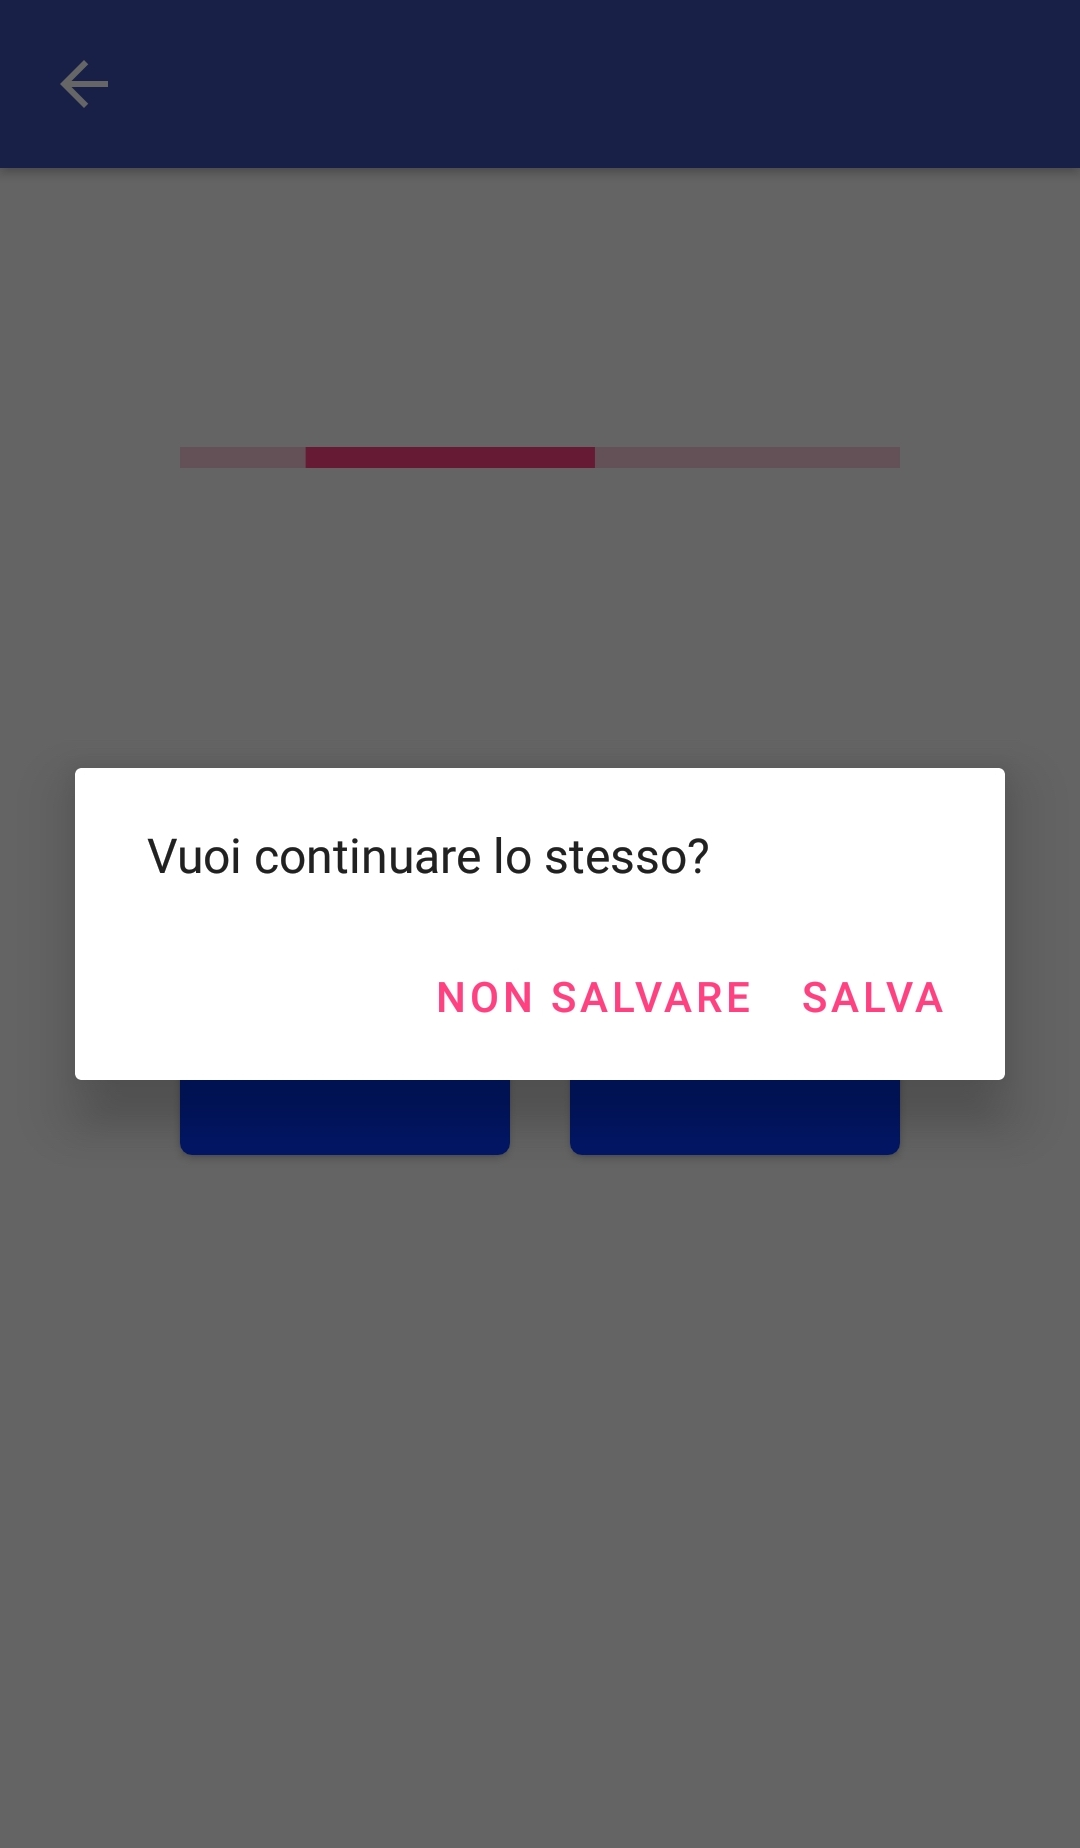
\includegraphics[scale=0.14]{Tesi/images/AlertVocale}
	\caption{\textit{Alert nota vocale e barra di progressione}}
	\label{fig:alertvocale}
\end{figure}
\\Sono presenti anche dei messaggi che avvisano l'utente nel caso in cui schiacci erroneamente sul bottone "Avvia" dopo che è già stata iniziata una registrazione, oppure sul bottone "Ferma" se non è stata ancora iniziata una registrazione.
\\Queste snackbar si possono osservare rispettivamente nelle figure \ref{fig:snackavvia} e \ref{fig:snackferma}:
\begin{figure}[!h]
    \centering
	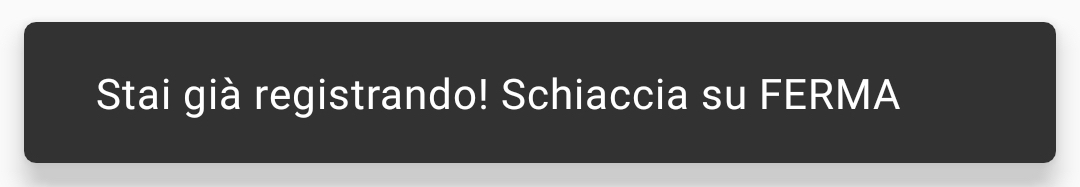
\includegraphics[scale=0.3]{Tesi/images/SnackAvvia.jpg}
	\caption{\textit{Snackbar tasto avvia}}
	\label{fig:snackavvia}
\end{figure}
\begin{figure}[!h]
    \centering
	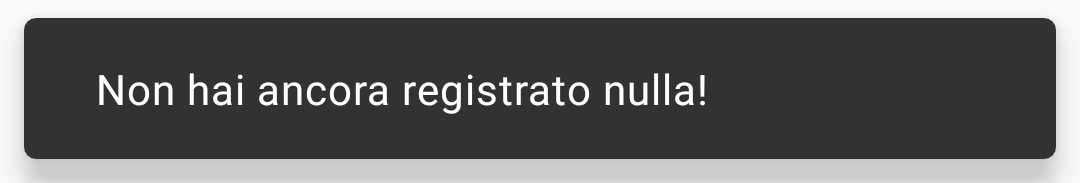
\includegraphics[scale=0.3]{Tesi/images/SnackFerma.jpg}
	\caption{\textit{Snackbar tasto ferma}}
	\label{fig:snackferma}
\end{figure}\pagebreak

\section{Nota Scritta}
\label{notascritta}
La schermata per inserire la nota scritta si presenta in questo modo, visibile in figura \ref{fig:notascritta}, che si riferisce al layout \textit{activity\_text\_note.xml}:
\begin{figure}[!h]
    \centering
	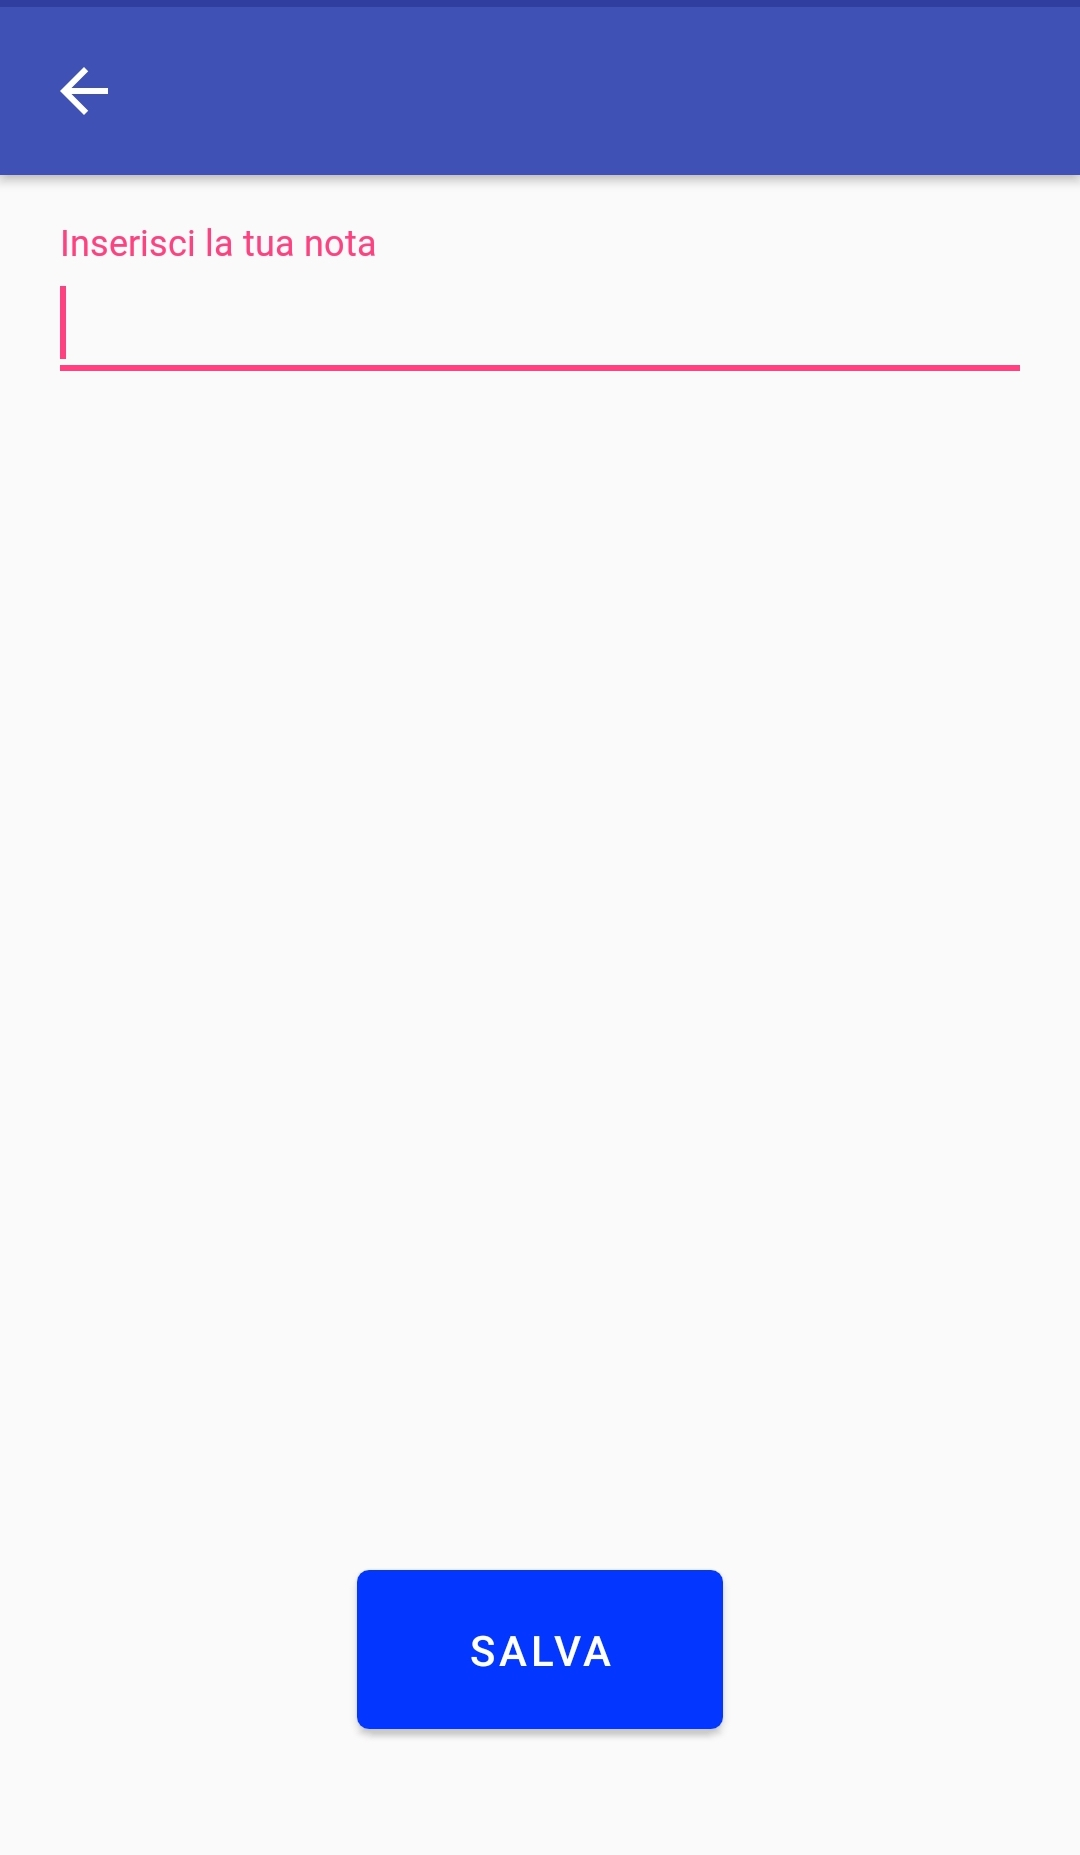
\includegraphics[scale=0.14]{Tesi/images/AttNota.jpg}
	\caption{\textit{Schermata per inserimento nota scritta}}
	\label{fig:notascritta}
\end{figure}
\\L'utente potrà inserire un testo, nel campo apposito, per poi salvare la nota, schiacciando sul bottone "Salva".
\\Una volta salvata la nota scritta, l'applicazione tornerà alla schermata precedente, visibile in figura \ref{fig:homepage}.
\\Se l'utente desiderasse modificare la nota, basterà schiacciare nuovamente sul bottone, nella schermata principale \ref{fig:homepage}, dedicato alla nota scritta, e troverà all'interno del campo di testo, ciò che aveva scritto in precedenza.
\\Se l'utente, invece, decidesse di tornare indietro senza salvare la nota scritta, verrà avvisato tramite un messaggio, che si può osservare in figura \ref{fig:alertnota}:
\begin{figure}[!h]
    \centering
	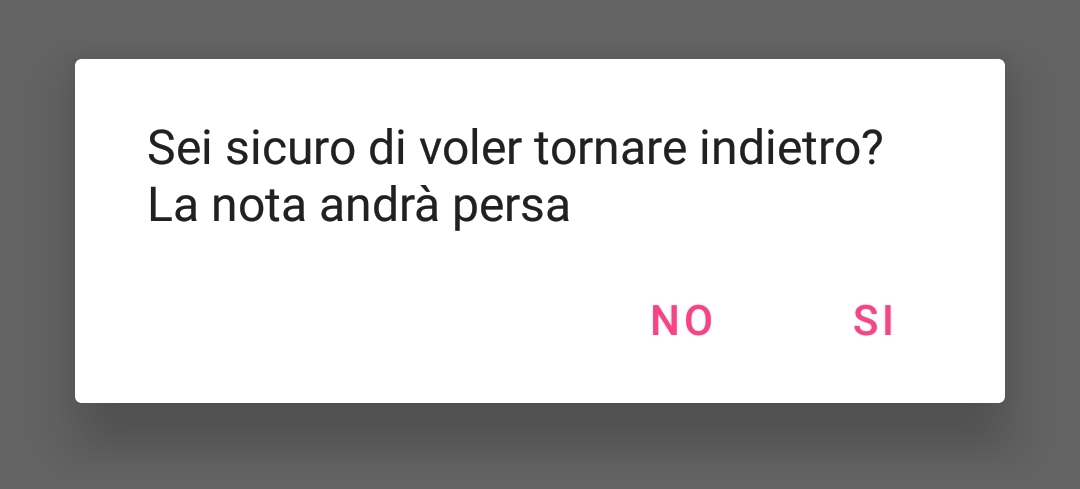
\includegraphics[scale=0.25]{Tesi/images/AlertNota}
	\caption{\textit{Alert mancato salvataggio nota scritta}}
	\label{fig:alertnota}
\end{figure}

\section{Modifica foto}
\label{modificafoto}
In questa schermata, accessibile schiacciando il bottone modifica visibile in figura \ref{fig:homepagemodifica} sotto l'icona delle foto, permette all'utente di cancellare una foto alla volta.
\\La schermata si presenta in questo modo in figura \ref{fig:modificafoto} e si riferisce al layout \textit{activity\_modify\_photo.xml}:
\begin{figure}[!h]
    \centering
	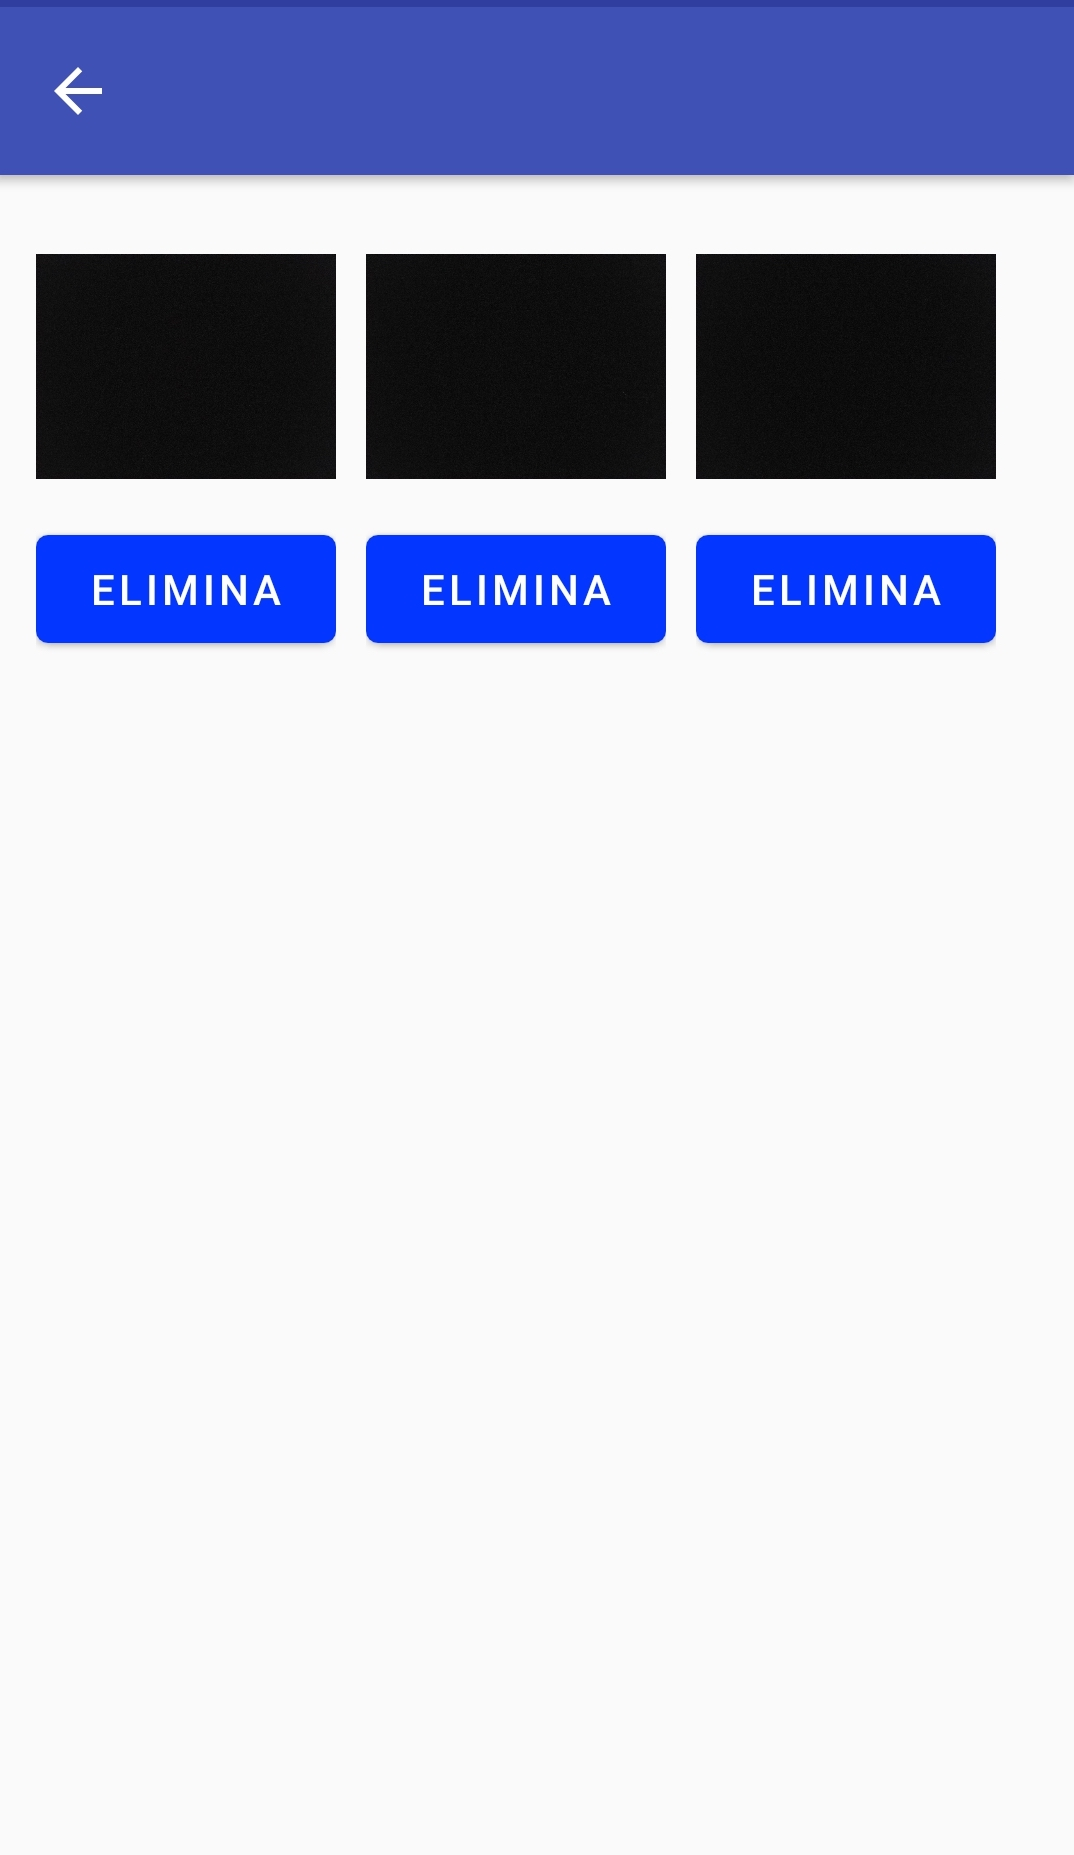
\includegraphics[scale=0.14]{Tesi/images/ModificaFoto.jpg}
	\caption{\textit{Schermata modifica foto}}
	\label{fig:modificafoto}
\end{figure}
\\Schiacciando sul bottone elimina, comparirà un messaggio, che avviserà l'utente se è effettivamente convinto di cancellare quella foto. Si presenta come in figura \ref{fig:alertfoto}:
\begin{figure}[!h]
    \centering
	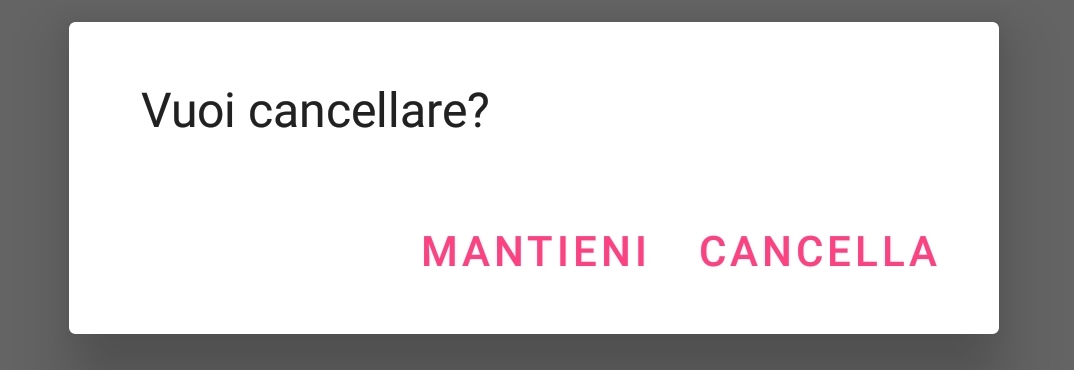
\includegraphics[scale=0.2]{Tesi/images/AlertFoto}
	\caption{\textit{Alert eliminazione foto}}
	\label{fig:alertfoto}
\end{figure}
\\A questo punto l'utente potrà decidere se mantenerla oppure cancellarla effettivamente. 
\\Se l'utente premerà il bottone "Mantieni" l'applicazione rimarrà nella schermata corrente. Se schiaccerà sul bottone "Cancella", verrà cancellata la foto ed a questo punto l'applicazione tornerà alla schermata precedente.\pagebreak

\section{Modifica video}
\label{modificavideo}
In questa schermata, accessibile schiacciando il bottone modifica visibile in figura \ref{fig:homepagemodifica} sotto l'icona dei video, permette all'utente di cancellare un video alla volta. Verrà illustrata l'anteprima del rispettivo video.
\\La schermata si presenta in questo modo in figura \ref{fig:modificavideo} e si riferisce al layout \textit{activity\_modify\_video.xml}:
\begin{figure}[!h]
    \centering
	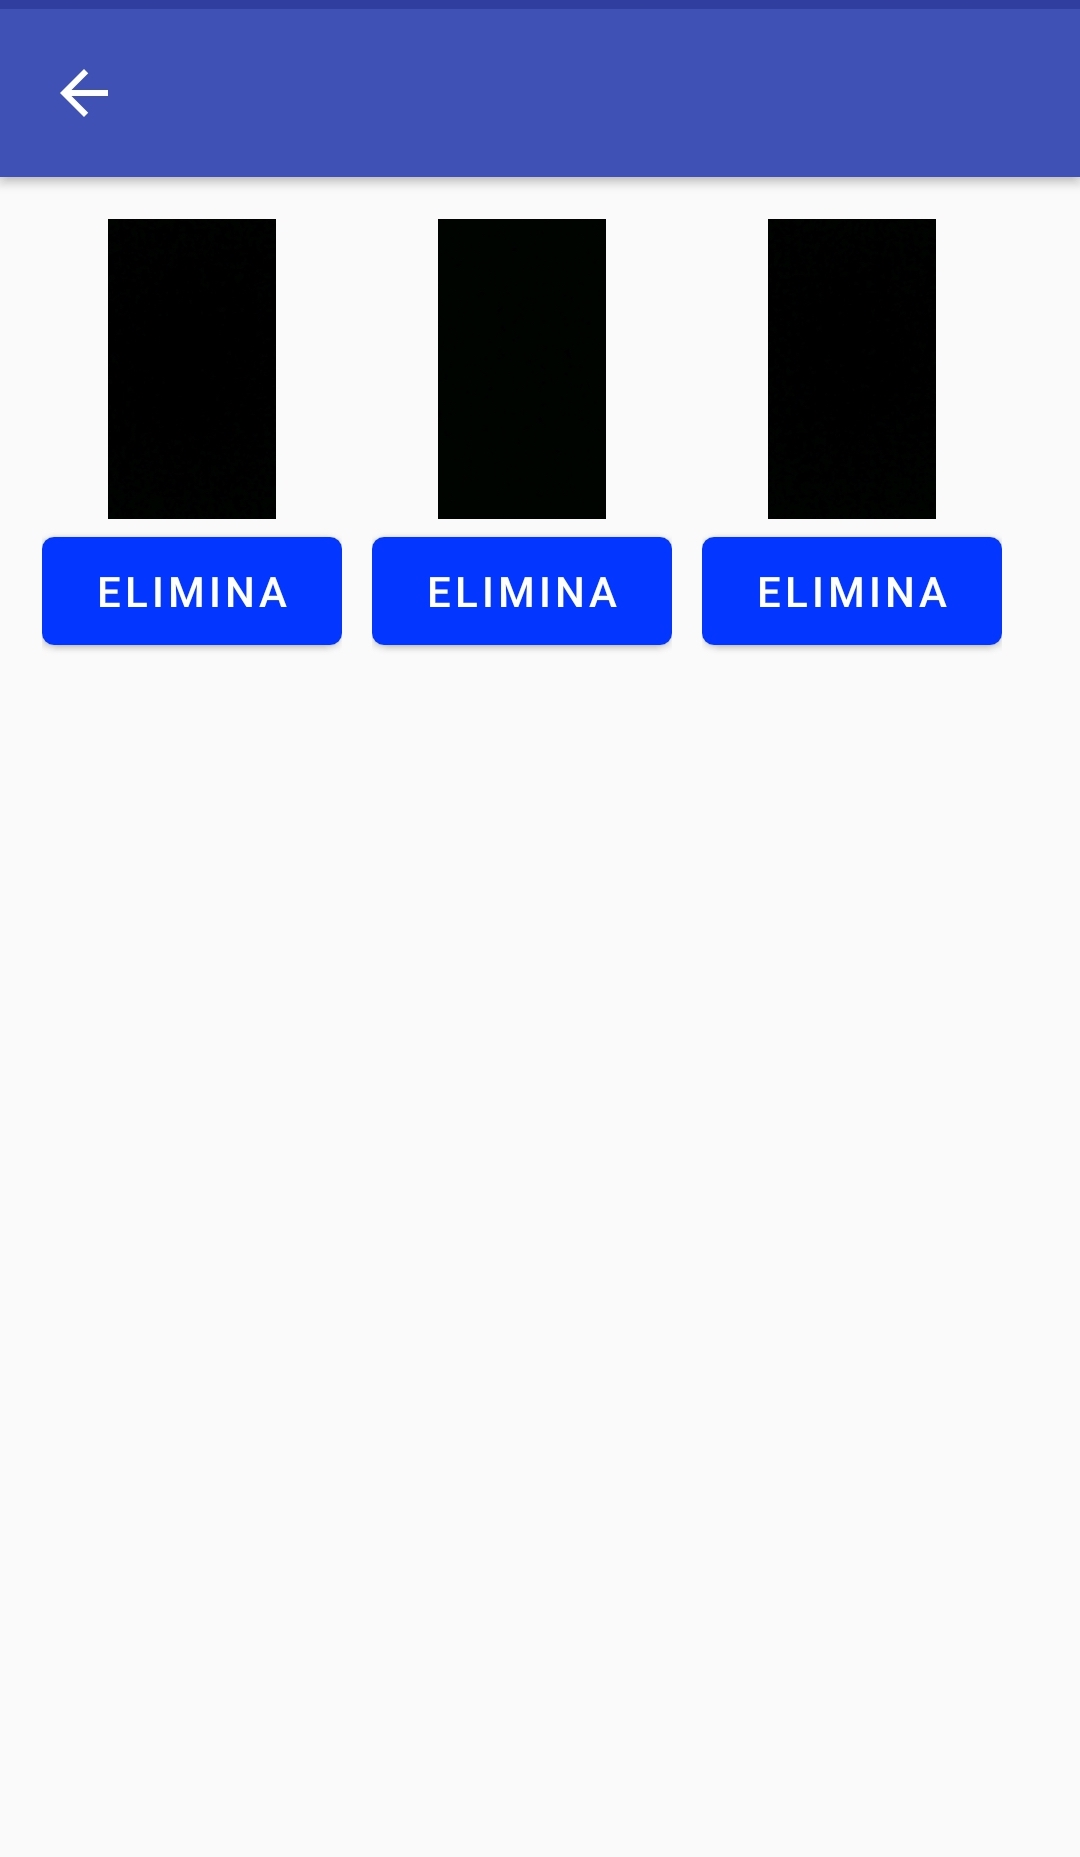
\includegraphics[scale=0.14]{Tesi/images/ModificaVideo.jpg}
	\caption{\textit{Schermata modifica video}}
	\label{fig:modificavideo}
\end{figure}
\\Schiacciando sul bottone "Elimina", comparirà un messaggio, che avviserà l'utente se è effettivamente convinto di cancellare quel video. Si presenta come in figura \ref{fig:alertfoto}:
\begin{figure}[!h]
    \centering
	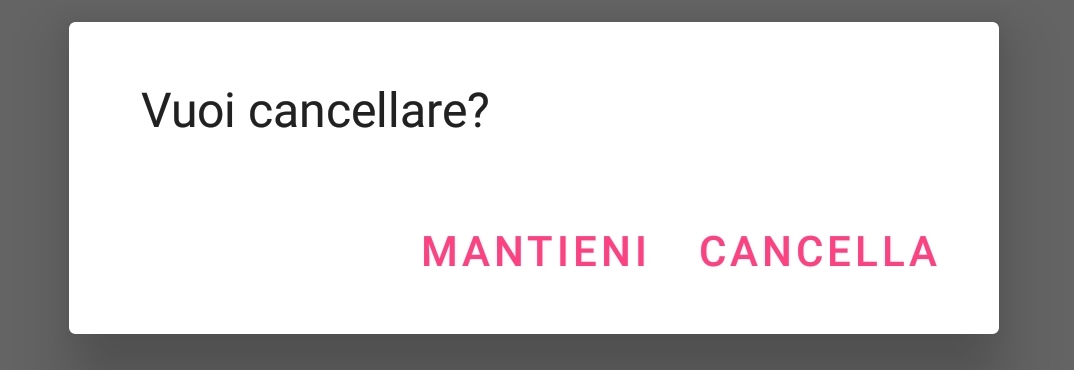
\includegraphics[scale=0.2]{Tesi/images/AlertFoto}
	\caption{\textit{Alert eliminazione video}}
	\label{fig:alertfoto}
\end{figure}
\\A questo punto l'utente potrà decidere se mantenerlo oppure cancellarlo effettivamente. 
\\Se l'utente premerà il bottone "Mantieni" l'applicazione rimarrà nella schermata corrente, se schiaccerà sul bottone "Cancella", verrà cancellato il video ed a questo punto l'applicazione tornerà alla schermata precedente.\pagebreak

\section{Modifica nota vocale}
\label{modificavocale}
In questa schermata, accessibile schiacciando il bottone modifica visibile in figura \ref{fig:homepagemodifica} sotto l'icona della nota vocale, permette all'utente di cancellare una nota vocale alla volta.
\\La schermata si presenta in questo modo in figura \ref{fig:modificavocale} e si riferisce al layout \textit{activity\_modify\_voice\_note.xml}:
\begin{figure}[!h]
    \centering
	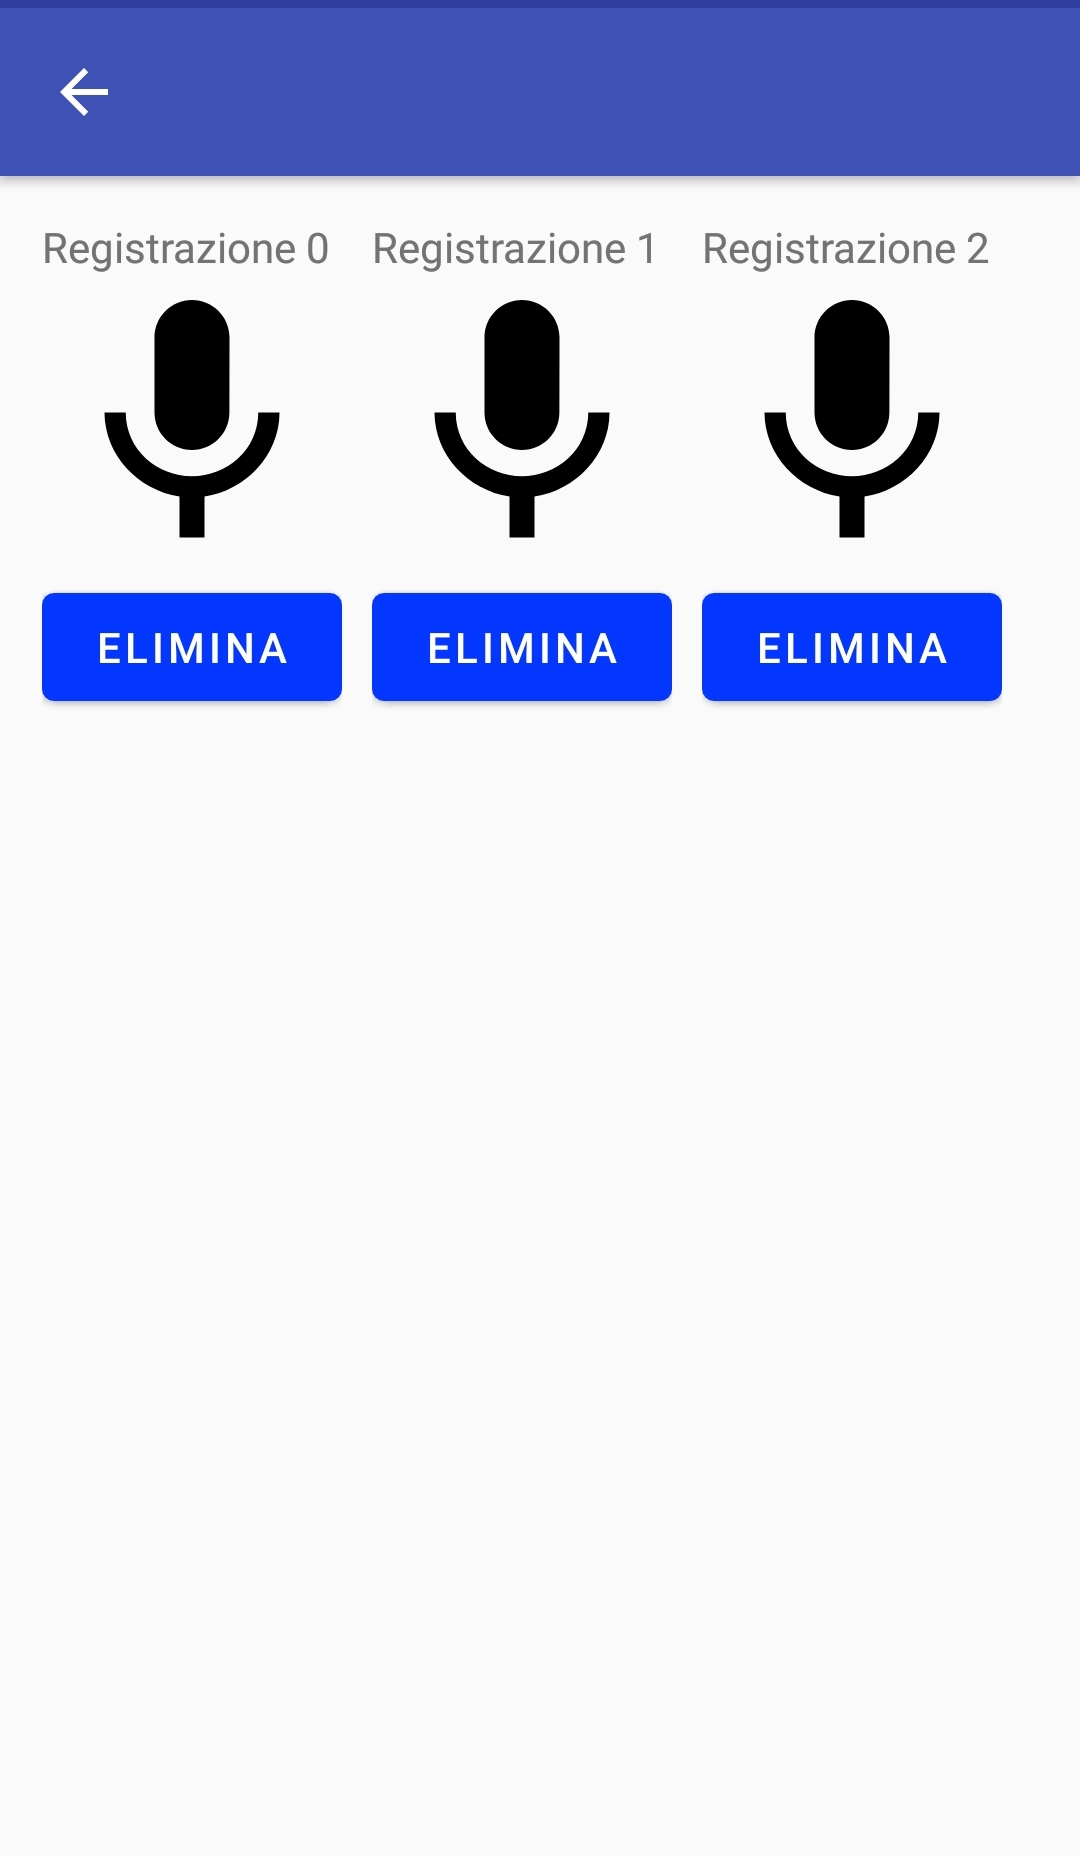
\includegraphics[scale=0.14]{Tesi/images/ModificaVocale.jpg}
	\caption{\textit{Schermata modifica nota vocale}}
	\label{fig:modificavocale}
\end{figure}
\\Schiacciando sul bottone "Elimina", comparirà un messaggio, che avviserà l'utente se è effettivamente convinto di cancellare quella nota vocale. Si presenta come in figura \ref{fig:alertfoto}:
\begin{figure}[!h]
    \centering
	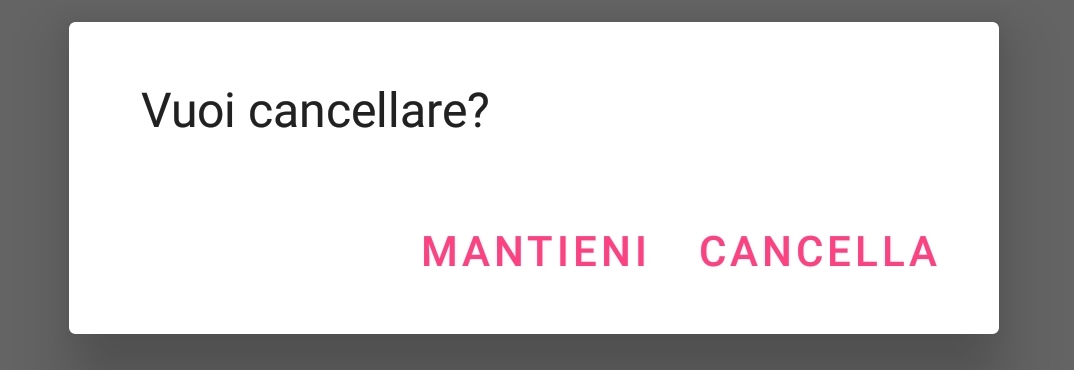
\includegraphics[scale=0.2]{Tesi/images/AlertFoto}
	\caption{\textit{Alert eliminazione video}}
	\label{fig:alertfoto}
\end{figure}
\\A questo punto l'utente potrà decidere se mantenerla oppure cancellarla effettivamente. 
\\Se l'utente premerà il bottone "Mantieni" l'applicazione rimarrà nella schermata corrente, se schiaccerà sul bottone "Cancella", verrà cancellata la nota vocale ed a questo punto l'applicazione tornerà alla schermata precedente.\pagebreak
